%---------------------------------------------------------
\chapter{Propuesta del proyecto}
%---------------------------------------------------------
\section{Análisis del problema}
\subsection{Problema general}
ESPECTACULARES S.A. de C.V. no es capaz de realizar la totalidad de sus procesos a través del sistema de administración de recursos empresariales (ERP) que actualmente posee.\par
\subsection{Problemas específicos}
\begin{itemize}
\item{El ERP de la empresa fue diseñado para contener la cartera de clientes. Sin embargo, no cuenta con la cartera de clientes completa ni con información actualizada.}
\item{El ERP de la empresa fue diseñado para contener la plantilla de empleado pero, tal y como sucede con la cartera de clientes, no se encuentra completa ni actualizada y no hay forma de distinguir empleados de un departamento que de otro.}
\item{La empresa refleja una pérdida de clientes de aproximadamente de entre 10 y 15 por año.}
\item{El gerente de ventas y sus agentes no pueden registrar las ventas y/ó cotizaciones de un cliente en el ERP.}
\item{Los agentes de ventas no son capaces de visualizar en el ERP las ventas y/ó cotizaciones que ha realizado con un cliente anteriormente.}
\item{El gerente de ventas no puede asignar ventas a un agente de ventas desde el ERP.}
\item{El titular de jurídico y sus agentes no son capaces de encontrar las pólizas y/o permisos de un determinado espectacular de manera eficiente (se busca en el archivo físico de cada agente cuando se requiere).}
\item{El jefe de infraestructura y sus agentes no son capaces de saber a ciencia cierta cuántos y cuáles espectaculares necesitan mantenimiento, de qué tipo (preventivo, correctivo).}
\item{El jefe de infraestructura y sus agentes no son capaces de saber a ciencia cierta cuántos y cuáles espectaculares están fuera de servicio (ya sea porque no pertenecen a la empresa, o están dañados).}
\item{La empresa no sabe a ciencia cierta cuántos y cuáles han sido los trabajos en conjunto que ha hecho con Publicidad ni las especificaciones de estos trabajos.}
\end{itemize}
\subsection{Causas}
\begin{itemize}
\item{Los únicos empleados con acceso al ERP son los procedentes del departamento de capital humano, sin embargo, ellos no se encargan de tratar con los clientes y tampoco mantienen actualizada la plantilla de empleados (debido a que no se sienten cómodos con el ERP).}
\item{Cada que un agente de ventas termina su relación laboral con la empresa, se lleva con él la cartera de clientes que le correspondía (dado que sólo él tenía trato con ellos y nadie más conocía los datos del cliente).}
\item{El ERP no está diseñado para registrar cotizaciones y/ó ventas.}
\item{El ERP no está diseñado para asignar cotizaciones y/ó ventas.}
\item{El ERP no está diseñado para registrar permisos y/ó pólizas ni mucho menos asociarlos a un espectacular.}
\item{El ERP no está diseñado para registrar espectaculares. Esto mismo impide el conocimiento de cualquier dato relacionado con un espectacular.}
\end{itemize}
\subsection{Consecuencias}
\begin{itemize}
\item{Pérdida de información.}
\item{Información registrada desactualizada.}
\item{Información registrada incompleta.}
\item{Pérdida de control de siniestros.}
\item{Pérdida de control de empleados.}
\item{Pérdida de control de clientes.}
\end{itemize}
%---------------------------------------------------------RUX
%---------------------------------------------------------
\subsection{Requerimientos de usuario}
Los requerimientos del usuario utilizan una clave RUX, donde:

\begin{description}
        \item[X] Es un número consecutivo: 1, 2, 3, ...
        \item[RU] Es la clave para todos los {\bf R}equerimientos del {\bf U}suario.
\end{description}
\newpage
Además se usan las abreviaciones que se muestran en la tabla~\ref{tbl:leyendaRU}.
\begin{table}[hbtp!]
        \begin{center}
    \begin{tabular}{|r l|}
            \hline
        {\footnotesize ID} & {\footnotesize\em Identificador del requerimiento.}\\
        {\footnotesize PRI.} & {\footnotesize\em Prioridad}\\
        {\footnotesize MA} & {\footnotesize\em Prioridad Muy Alta.}\\
        {\footnotesize A} & {\footnotesize\em Prioridad Alta.}\\
        {\footnotesize M} & {\footnotesize\em Prioridad Media.}\\
        {\footnotesize B} & {\footnotesize\em Prioridad Baja.}\\
        {\footnotesize MB} & {\footnotesize\em Prioridad Muy Baja.}\\
                \hline
    \end{tabular} 
    \caption{Leyenda para los requerimientos de usuario.}
    \label{tbl:leyendaRU}
        \end{center}
\end{table}

En la tabla ~\ref{tbl:listaRU} se muestran los requerimientos de usuario que se tomaron en cuenta para la realización de esta propuesta.

\begin{longtable}[H]{m{1cm}m{3cm}m{10cm}m{1cm}}
\toprule
\centering \textbf{ID} & \centering  \textbf{Nombre} & \centering \textbf{Descripción} & \centering \textbf{PRI} \tabularnewline
\midrule
\textit{RU1} &\textbf{Visualización de detalles de arrendamiento} & El cliente requiere de la correcta visualización de los detalles (fecha de inicio del contrato de renta, fecha de término del contrato de renta, número de espectaculares, número de contrato de renta, precio pactado en el contrato de renta) de cada uno de los espectaculares  de los cuales firmó un contrato de arrendamiento con la empresa. (hasta 1 año atrás, y los que  tenga rentados en el momento de la petición). & B\tabularnewline
\textit{RU2} &\textbf{Solicitud de renovación contrato} & El cliente requiere una solicitud de renovación del contrato de renta a la empresa. & MB\tabularnewline
\textit{RU3} &\textbf{Solicitud presupuesto} & El cliente requiere solicitar un presupuesto de contrato de renta. & MB\tabularnewline
\textit{RU4} &\textbf{Notificación renovación contrato} & El cliente debe ser notificado acerca de la respuesta a su solicitud de renovación del contrato de renta por la empresa al menos 3 días hábiles antes de  que inicie el nuevo período de renta. & MB\tabularnewline
\textit{RU5} &\textbf{Notificación presupuesto} & El cliente necesita ser notificado acerca de la respuesta  a su solicitud de presupuesto de renta por la empresa como máximo 3 días hábiles después de que éste la elaboró. &\tabularnewline
\textit{RU6} &\textbf{Facturación} & El cliente requiere facturar cada uno de los contratos de renta que firme con la empresa en el año fiscal vigente. & MB\tabularnewline
\textit{RU7} &\textbf{Plantilla agentes de ventas} & El gerente de ventas requiere saber cuántos y cuáles son los agentes de ventas que están registrados en su plantilla de trabajo (de manera correcta y actualizada), así como sus datos personales (nombre completo, teléfono fijo, teléfono celular, dirección, correo electrónico). & MA\tabularnewline
\textit{RU8} &\textbf{Listas de ventas asignadas} & El gerente de ventas necesita saber (de manera correcta y actualizada) los clientes que ya han sido asignados a un agente de ventas. & A\tabularnewline
\textit{RU9} &\textbf{Lista de ventas pendientes} & El gerente de ventas necesita saber (de manera correcta y actualizada) los cliente que quedan por asignar. &\tabularnewline
\textit{RU10} &\textbf{Asignar ventas pendientes} & El gerente de ventas necesita asignar clientes pendientes a cada uno de los agentes de ventas. & A\tabularnewline
\textit{RU11} &\textbf{Alta clientes gerencia} & El gerente de ventas requiere almacenar los datos personales a un cliente (nombre completo, teléfono fijo, teléfono celular, dirección, correo electrónico, rfc). & MA\tabularnewline
\textit{RU12} &\textbf{Lista clientes} & El gerente de ventas necesita conocer cuántos y cuáles son los clientes han realizado transacciones en el pasado (hasta 1 año atrás) y/o en el presente con la empresa, y sus datos personales.  & MA\tabularnewline
\textit{RU13} &\textbf{Cambios clientes gerencia} & El gerente de ventas requiere actualizar a los datos personales de un cliente. & MA\tabularnewline
\textit{RU14} &\textbf{Eliminación cliente} & El gerente de ventas necesita poder eliminar los datos personales de un cliente para evitar confusiones con los agentes de ventas. Sin embargo, requiere almacenar sus datos para cualquier aclaración. & A\tabularnewline
\textit{RU15} &\textbf{Eliminación agente de ventas} & El gerente de ventas necesita eliminar los datos personales de un ex-agente de ventas para no considerarle para asignación de clientes. Sin embargo, requiere poder tener a la mano dichos datos para cualquier aclaración. & MA\tabularnewline
\textit{RU16} &\textbf{Listado clientes sin agente de ventas} & El gerente de ventas necesita saber cuántos y cuáles son los clientes que tenían asignado un agente de ventas que se ha eliminado de la plantilla de trabajos, para atenderlos él mismo o asignarle un nuevo agente de ventas. & MA\tabularnewline
\textit{RU17} &\textbf{Listado cientes por gerente ventas} & El agente de ventas necesita conocer cuántos y cuáles son los clientes han realizado transacciones en el pasado (hasta 1 año atrás) y/o en el presente con él, y sus datos personales. & A\tabularnewline
\textit{RU18} &\textbf{Alta clientes agente} & El agente de ventas requiere anotar los datos personales a un cliente (nombre completo, teléfono fijo, teléfono celular, dirección, correo electrónico, rfc). & A\tabularnewline
\textit{RU19} &\textbf{Cambios clientes agente} & El agente de ventas necesita actualizar los datos personales de un cliente. & A\tabularnewline
\textit{RU20} &\textbf{Presupuestos agente} & El agente de ventas necesita realizar presupuestos para los distintos clientes que atiende de acuerdo a sus necesidades (grado de impacto, medidas, medio, vistas, ubicación, tipo y precio). & A\tabularnewline
\textit{RU21} &\textbf{Presupuestos gerente} & El gerente de ventas necesita realizar presupuestos para los distintos cliente que atiende de acuerdo a sus necesidades (grado de impacto, medidas, medio, vistas, ubicación, tipo y precio). &\tabularnewline
\textit{RU22} &\textbf{Confirmación presupuesto agente} & El agente de ventas debe confirmar los presupuestos de los clientes que hayan aceptado éstos. & A\tabularnewline
\textit{RU23} &\textbf{Confirmación presupuesto gerente} & El gerente de ventas debe confirmar los presupuestos de los clientes que hayan aceptado éstos. & MA\tabularnewline
\textit{RU24} &\textbf{Presupuestos pendientes gerente} & El gerente de ventas requiere conocer cuántos y cuáles son los presupuestos que se encuentran en plazo de tolerancia y a qué cliente pertenece. & MA\tabularnewline
\textit{RU25} &\textbf{Presupuestos pendientes agente} & El agente de ventas requiere conocer cuántos y cuáles son los presupuestos que se encuentran en plazo de tolerancia y a qué cliente pertenece. & A\tabularnewline
\textit{RU26} &\textbf{Cancelar presupuestos gerente} & El gerente de ventas requiere cancelar los presupuestos de los clientes que no hayan llegado a ningún acuerdo con éste después del plazo de tolerancia. & MA\tabularnewline
\textit{RU27} &\textbf{Cancelar presupuestos agente} & El agente de ventas debe cancelar los presupuestos de los clientes que no hayan llegado a ningún acuerdo con éste después del plazo de tolerancia. & A \tabularnewline
\textit{RU28} &\textbf{Listado permisos SSP titular} & El titular de jurídico requiere saber cuántos y cuáles espectaculares tienen vigente el permiso de la SSP correspondiente y los datos asociados a este (número de permiso, período de vigencia del permiso y agente jurídico que tramitó el permiso) que están registrados en su plantilla de espectaculares (de manera correcta y actualizada). & MA\tabularnewline
\textit{RU29} &\textbf{Listado permisos SPC titular} & El titular de jurídico requiere saber cuántos y cuáles espectaculares tienen vigente el permiso de SPC correspondiente y los datos asociados a este (número de permiso, período de  vigencia del permiso y agente jurídico que tramitó el permiso) que están registrados en su plantilla de espectaculares (de manera correcta y actualizada). & MA\tabularnewline
\textit{RU30} &\textbf{Listado pólizas titular} & El titular de jurídico requiere saber cuántos y cuáles espectaculares tienen vigente la póliza de seguros correspondiente y los datos asociados a este (aseguradora, número de póliza, período de vigencia de la póliza, qué cubre la póliza y por cuánto, y agente jurídico que tramitó la póliza) que están registrados en su plantilla de espectaculares (de manera correcta y actualizada). & MA\tabularnewline
\textit{RU31} &\textbf{Listado permisos SOBSE titular} & El titular de jurídico requiere saber cuántos y cuáles espectaculares tienen vigente el permiso de SOBSE correspondiente y los datos asociados a este (número de permiso, período de  vigencia del permiso y agente jurídico que tramitó el permiso) que están registrados en su plantilla de espectaculares (de manera correcta y actualizada). & MA\tabularnewline
\textit{RU32} &\textbf{Alta permiso SSP titular} & El titular de jurídico requiere dar de alta un nuevo permiso de la SSP asociado a un espectacular y sus respectivos datos (número de permiso (número de permiso, fecha de inicio de cobertura del permiso , fecha de término de cobertura del permiso, estado y agente jurídico que tramitó dicho permiso) & MA\tabularnewline
\textit{RU33} &\textbf{Alta permiso SPC titular} & El titular de jurídico requiere dar de alta un nuevo permiso de la SPC asociado a un espectacular y sus respectivos datos (número de permiso (número de permiso, fecha de inicio de cobertura del permiso , fecha de término de cobertura del permiso, estado y agente jurídico que tramitó dicho permiso) & MA\tabularnewline
\textit{RU34} &\textbf{Alta póliza titular} & El titular de jurídico requiere dar de alta un nuevo permiso de la SPC asociado a un espectacular y sus respectivos datos (nombre de la aseguradora contratada, número de póliza, fecha de inicio de cobertura de la póliza, fecha de término de cobertura de la póliza, cobertura de la póliza, estado y agente jurídico que tramitó dicha póliza) & MA\tabularnewline
\textit{RU35} &\textbf{Alta permiso SOBSE titular} & El titular de jurídico requiere dar de alta un nuevo permiso de la SOBSE asociado a un espectacular y sus respectivos datos (número de permiso (número de permiso, fecha de inicio de cobertura del permiso , fecha de término de cobertura del permiso, estado y agente jurídico que tramitó dicho permiso) & MA\tabularnewline
\textit{RU36} &\textbf{Cambios permiso SSP titular} & El titular de jurídico debe actualizar los datos de un permiso de la SSP asociado a un espectacular. & MA\tabularnewline
\textit{RU37} &\textbf{Cambios permiso SPC titular} & El titular de jurídico debe actualizar en los datos de un permiso de la SPC asociado a un espectacular. & MA\tabularnewline
\textit{RU38} &\textbf{Cambios póliza titular} & El titular de jurídico debe actualizar en los datos de una póliza asociado a un espectacular. & MA\tabularnewline
\textit{RU39} &\textbf{Cambios permiso SOBSE titular} & El titular de jurídico debe actualizar en los datos de un permiso de la SOBSE asociado a un espectacular. & MA\tabularnewline
\textit{RU40} &\textbf{Eliminación permiso SSP} & El titular de jurídico necesita eliminar la de un permiso vencido de la SSP asociado a un espectacular. Sin embargo, también requiere un registro de dicha información para aclaraciones. & MA\tabularnewline
\textit{RU41} &\textbf{Eliminación permiso SPC} & El titular de jurídico necesita eliminar la de un permiso vencido de la SPC asociado a un espectacular. Sin embargo, también requiere un registro de dicha información para aclaraciones.. & MA\tabularnewline
\textit{RU42} &\textbf{Eliminación póliza} & El titular de jurídico necesita eliminar una póliza de seguros vencida asociada a un espectacular. Sin embargo, también requiere un registro de dicha información para aclaraciones. & MA\tabularnewline
\textit{RU43} &\textbf{Eliminación permiso SOBSE} & El titular de jurídico necesita eliminar la de un permiso vencido de la SOBSE asociado a un espectacular. Sin embargo, también requiere un registro de dicha información para aclaraciones. & MA\tabularnewline
\textit{RU44} &\textbf{Listado permisos SSP agente} & El agente jurídico requiere saber cuántos y cuáles espectaculares tienen vigente el permiso de la SSP correspondiente y los datos asociados a este (número de permiso, período de vigencia del permiso y agente jurídico que tramitó el permiso) que están registrados en su plantilla de espectaculares (de manera correcta y actualizada). & A\tabularnewline
\textit{RU45} &\textbf{Listado permisos SPC agente} & El agente jurídico requiere saber cuántos y cuáles espectaculares tienen vigente el permiso de SPC correspondiente y los datos asociados a este (número de permiso, período de  vigencia del permiso y agente jurídico que tramitó el permiso) que están registrados en su plantilla de espectaculares (de manera correcta y actualizada). & A\tabularnewline
\textit{RU46} &\textbf{Listado pólizas agente} & El agente jurídico requiere saber cuántos y cuáles espectaculares tienen vigente la póliza de seguros correspondiente y los datos asociados a este (aseguradora, número de póliza, período de vigencia de la póliza, qué cubre la póliza y por cuánto, y agente jurídico que tramitó la póliza) que están registrados en su plantilla de espectaculares (de manera correcta y actualizada). & A\tabularnewline
\textit{RU47} &\textbf{Listado permisos SOBSE agente} & El agente jurídico requiere saber cuántos y cuáles espectaculares tienen vigente el permiso de SOBSE correspondiente y los datos asociados a este (número de permiso, período de  vigencia del permiso y agente jurídico que tramitó el permiso) que están registrados en su plantilla de espectaculares (de manera correcta y actualizada). & A\tabularnewline
\textit{RU48} &\textbf{Alta permiso SSP agente} & El agente jurídico necesita almacenar la información correspondiente a un nuevo permiso de la SSP asociado a un espectacular y sus respectivos datos (número de permiso (número de permiso, fecha de inicio de cobertura del permiso , fecha de término de cobertura del permiso, estado y agente jurídico que tramitó dicho permiso) & A\tabularnewline
\textit{RU49} &\textbf{Alta permiso SPC agente} & El agente jurídico necesita almacenar la información correspondiente a un nuevo permiso de la SPC asociado a un espectacular y sus respectivos datos (número de permiso (número de permiso, fecha de inicio de cobertura del permiso , fecha de término de cobertura del permiso, estado y agente jurídico que tramitó dicho permiso) & A\tabularnewline
\textit{RU50} &\textbf{Alta póliza agente} & El agente jurídico requiere necesita almacenar la información correspondiente a un nuevo permiso de la SPC asociado a un espectacular y sus respectivos datos (nombre de la aseguradora contratada, número de póliza, fecha de inicio de cobertura de la póliza, fecha de término de cobertura de la póliza, cobertura de la póliza, estado y agente jurídico que tramitó dicha póliza) & A\tabularnewline
\textit{RU51} &\textbf{Alta permiso SOBSE agente} & El agente jurídico necesita almacenar la información correspondiente a un nuevo permiso de la SOBSE asociado a un espectacular y sus respectivos datos (número de permiso (número de permiso, fecha de inicio de cobertura del permiso , fecha de término de cobertura del permiso, estado y agente jurídico que tramitó dicho permiso) & A\tabularnewline
\textit{RU52} &\textbf{Cambios permiso SSP agente} & El agente jurídico requiere actualizar los datos de un permiso de la SSP asociado a un espectacular. & A\tabularnewline
\textit{RU53} &\textbf{Cambios permiso SPC agente} & El agente jurídico requiere actualizar en los datos de un permiso de la SPC asociado a un espectacular. & A\tabularnewline
\textit{RU54} &\textbf{Cambios póliza agente} & El agente jurídico requiere hacer actualizar en los datos de una póliza asociado a un espectacular. & A\tabularnewline
\textit{RU55} &\textbf{Cambios permiso SOBSE agente} & El agentejurídico requiere actualizar en los datos de un permiso de la SOBSE asociado a un espectacular. & A
\tabularnewline
\textit{RU56} & \textbf{Listado plantilla empleados} & El jefe de capital humano requiere saber cuántos y cuáles son los empleados registrados en la plantilla de la empresa (de todos los departamentos) así como sus datos personales (nombre completo, teléfono fijo, teléfono celular, dirección, correo electrónico, departamento al que pertenece, puesto). & MA\tabularnewline
\textit{RU57} & \textbf{Alta nuevo empleado titular} & El jefe de capital humano requiere registrar los datos de un nuevo empleado en la plantilla de la empresa (de cualesquiera que sea su departamento y/o cargo), ingresando sus datos personales (nombre completo, dirección, teléfono fijo, teléfono celular, dirección de correo electrónico, situación, departamento y tipo de empleado.\ & MA\tabularnewline
\textit{RU58} & \textbf{Cambio empleado titular} & El jefe de capital humano requiere modificar los datos asociados a un empleado registrado en la plantilla. & MA\tabularnewline
\textit{RU59} & \textbf{Eliminación empleado} & El jefe de capital humano requiere realizar la eliminación lógica de los datos de un empleado de la plantilla. & MA \tabularnewline
\textit{RU60} & \textbf{Copia listado plantilla empleados} & El agente de capital humano requiere saber cuántos y cuáles son los empleados registrados en la plantilla de la empresa (de todos los departamentos) así como sus datos personales (nombre completo, teléfono fijo, teléfono celular, dirección, correo electrónico, departamento al que pertenece, puesto). & A\tabularnewline
\textit{RU61} & \textbf{Alta nuevo empleado agente} & El agente de capital humano requiere almacenar los datos de un nuevo empleado en la plantilla de la empresa (de cualesquiera que sea su departamento y/o cargo), ingresando sus datos personales (nombre completo, dirección, teléfono fijo, teléfono celular, dirección de correo electrónico, situación, departamento y tipo de empleado.\ & A\tabularnewline
\textit{RU62} & \textbf{Cambio empleado agente} & El agente de capital humano requiere modificar los datos asociados a un empleado registrado en la plantilla. & A\tabularnewline
\textit{RU63} & \textbf{Alta espectacular jefe} & El jefe de infraestructura necesita almacenar los datos de un nuevo espectacular en la plantilla y sus datos asociados (ubicación en coordenadas, dirección de la ubicación, estado, fecha de inicio de contrato de arrendamiento, fecha de término de contrato de arrendamiento, categoría del espectacular, impacto promedio, medio, vistas, iluminación y medidas). & MA\tabularnewline
\textit{RU64} & \textbf{Listado espectaculares jefe} & El jefe de infraestructura requiere saber cuántos y cuáles son los espectaculares que están registrados (de manera correcta y actualizada), así como sus datos asociados. & MA\tabularnewline
\textit{RU65} & \textbf{Cambio espectacular jefe} & El jefe de infraestructura requiere realizar cambios en los datos asociados a un espectacular. & MA\tabularnewline
\textit{RU66} & \textbf{Eliminación espectacular} & El jefe de infraestructura debe eliminar los datos de un espectacular para que éste no sea tomado en cuenta para futuras ventas. Sin embargo, requiere tener un registro de estos datos para aclaraciones futuras. & MA\tabularnewline
\textit{RU67} & \textbf{Estado mantenimiento} & El jefe de infraestructura requiere ser notificado del estado de mantenimiento de cada espectacular registrado en la plantilla de la empresa antes de que éste requiera mantenimiento preventivo (3 días antes mínimo), o mantenimiento correctivo (en el momento exacto). & A\tabularnewline
\textit{RU68} & \textbf{Miembros cuadrilla jefe} & El jefe de infraestructura necesita conocer cuántos y cuáles agentes de infraestructura pertenecen a una cuadrilla de mantenimiento específica. & M\tabularnewline
\textit{RU69} & \textbf{Ubicación cuadrilla} & El jefe de infraestructura necesita conocer la ubicación en tiempo real de una cuadrilla. & M \tabularnewline
\textit{RU70} & \textbf{Asignar servicio} & El jefe de infraestructura necesita asignar a una cuadrilla un servicio de estimación de daños, mantenimiento, instalación o desmontaje dependiendo de su ubicación en tiempo real. & A\tabularnewline
\textit{RU71} & \textbf{Servicio realizado jefe} & El jefe de infraestructura necesita saber en tiempo real si un servicio de mantenimiento, estimación de daños, instalación o desmontaje ha sido realizado por la cuadrilla asignada. & A\tabularnewline
\textit{RU72} & \textbf{Alta espectacular jefe} & El jefe de infraestructura necesita poder dar de alta un nuevo espectacular en la plantilla y sus datos asociados (ubicación en coordenadas, dirección de la ubicación, estado, fecha de inicio de contrato de arrendamiento, fecha de término de contrato de arrendamiento, categoría del espectacular, impacto promedio, medio, vistas, iluminación y medidas). & MA\tabularnewline
\textit{RU73} & \textbf{Listado espectaculares líder} & El líder de cuadrilla requiere saber cuántos y cuáles son los espectaculares que están registrados (de manera correcta y actualizada), así como sus datos asociados. & A\tabularnewline
\textit{RU74} & \textbf{Cambio espectacular líder} & El líder de cuadrilla requiere realizar cambios en los datos asociados a un espectacular. & A\tabularnewline
\textit{RU75} & \textbf{Miembros cuadrilla líder} & El líder de una cuadrilla necesita conocer cuántos y cuáles agentes de infraestructura pertenecen a su cuadrilla. & M\tabularnewline
\textit{RU76} & \textbf{Servicio realizado líder} & El líder de cuadrilla necesita notificar en tiempo real si un servicio de mantenimiento, estimación de daños, instalación o desmontaje ha sido realizado por su cuadrilla & A\tabularnewline
\textit{RU77} & \textbf{Notificación siniestro jurídico} & El titular de jurídico requiere ser notificado en el momento exacto en que el jefe de infraestructura sea avisado de que ocurrió un siniestro en un espectacular. & MA\tabularnewline
\textit{RU78} & \textbf{Asignación siniestro jurídico} & El titular jurídico requiere notificar al agente jurídico encargado del trámite de los permisos y la póliza del espectacular que ha sufrido un siniestro. & MA\tabularnewline
\textit{RU79} & \textbf{Notificación siniestro agente jurídico} & El agente jurídico encargado de los permisos y la póliza del espectacular que ha sufrido un percance debe ser notificado para acudir al lugar de los hechos. & A\tabularnewline
\textit{RU80} & \textbf{Alta espectacular líder} & El líder de cuadrilla necesita poder almacenar los datos de un nuevo espectacular en la plantilla y sus datos asociados. & A\tabularnewline
\textit{RU81} & \textbf{Lista espectaculares ventas gerente} & El gerente de ventas necesita conocer lista de espectaculares con los que cuenta la empresa para poder considerarlo en un presupuesto o contrato de arrendamiento. & A\tabularnewline
\textit{RU82} & \textbf{Lista espectaculares ventas agente} & El agente de ventas necesita conocer la lista de espectaculares con los que cuenta la empresa para poder considerarlo en un presupuesto o contrato de arrendamiento. & A\tabularnewline
\textit{RU83} & \textbf{Generación de reporte de ventas} & El gerente de ventas requiere realizar un reporte de las ventas concretadas durante el mes en curso. & A\tabularnewline
\textit{RU84} & \textbf{Generación de reporte de clientes} & El gerente de ventas requiere realizar un reporte de las clientes que han actualizado sus datos en el mes en curso. & A\tabularnewline
\textit{RU85} & \textbf{Generación de reporte de empleados} & El jefe de capital humano requiere realizar un reporte de las actividades realizadas por cada empleado durante el mes para pago de bonos de productividad. & A\tabularnewline
\textit{RU86} & \textbf{Generación de reporte de siniestros} & El jefe de infraestructura requiere realizar un reporte de los siniestros ocurridos durante el mes en curso. & A\tabularnewline
\bottomrule
\caption{Requerimientos de usuario}
\label{tbl:listaRU}

\end{longtable}

%---------------------------------------------------------
\newpage
\section{Propuesta de solución}
\subsection{Objetivo general}
Diseñar un sistema de software disponible para dispositivos móviles y de escritorio; que funja como auxiliar en los procesos de ingreso, actualización y eliminación de información relacionada con los espectaculares, empleados, clientes, pólizas y permisos con el nivel de abstracción correspondiente al usuario que requiera estas acciones, así como permita la visualización de éstos cambios.
\subsection{Objetivos específicos}
\begin{itemize}
\item{Implementar el proceso de ingreso de espectaculares realizado por la empresa en su más básico escenario.}
\item{Implementar el proceso de actualización de espectaculares realizado por la empresa en su más básico escenario.}
\item{Implementar el proceso de eliminación de espectaculares realizado por la empresa en su más básico escenario.}
\item{Implementar el proceso de ingreso de empleados realizado por la empresa en su más básico escenario.}
\item{Implementar el proceso de actualización de empleados realizado por la empresa en su más básico escenario.}
\item{Implementar el proceso de eliminación de empleados realizado por la empresa en su más básico escenario.}
\item{Implementar el proceso de ingreso de clientes realizado por la empresa en su más básico escenario.}
\item{Implementar el proceso de actualización de clientes realizado por la empresa en su más básico escenario.}
\item{Implementar el proceso de eliminación de clientes realizado por la empresa en su más básico escenario.}
\item{Implementar el proceso de ingreso de permisos (de cualesquiera que se trate llámese de SSP, SPC, SOBSE) realizado por la empresa en su más básico escenario.}
\item{Implementar el proceso de actualización de permisos (de cualesquiera que se trate llámese de SSP, SPC, SOBSE) realizado por la empresa en su más básico escenario.}
\item{Implementar el proceso de eliminación de permisos (de cualesquiera que se trate llámese de SSP, SPC, SOBSE) realizado por la empresa en su más básico escenario.}
\item{Implementar el proceso de ingreso de pólizas realizado por la empresa en su más básico escenario.}
\item{Implementar el proceso de actualización de pólizas realizado por la empresa en su más básico escenario.}
\item{Implementar el proceso de eliminación de pólizas realizado por la empresa en su más básico escenario.}
\item{Implementar las restricciones necesarias para que se cumplan los estándares de cada uno de los procesos de la empresa.}
\item{Permitir la visualización de los datos de uno o varios espectaculares.}
\item{Permitir la visualización de los datos de uno o varios empleados.}
\item{Permitir la visualización de los datos de uno o varios permisos.}
\item{Permitir la visualización de los datos de uno o varios pólizas.}
\end{itemize}
\subsection{Descripción de la solución}
La presente propuesta desarrollará un sistema de software que permita gestionar adecuadamente la información de ESPECTACULARES S.A. de C.V.. El uso de este sistema de gestión se puede dividir de la siguiente manera:
\begin{itemize}
\item[1]{\textbf{Identificación de usuario}: El usuario debe iniciar sesión en el sistema con sus credenciales. Con esto, el mostrará una vista determinada por su tipo de usuario.}
\item[2]{\textbf{Despliegue de acciones de usuario}: Dependiendo del tipo de usuario identificado, el sistema mostrará una lista de acciones que éste puede llevar a cabo, como se enumeran a continuación:
	\begin{itemize}
	\item{\textit{Jefe}: Altas, cambios (inluyendo eliminación lógica), y consultas. Todo esto correspondiente a su departamento (espectaculares para infraestructura, agentes de ventas y clientes para ventas, permisos y pólizas para jurídico y empleados de su propio y otros departamentos para capital humano).}
	\item{\textit{Agente}: Altas, cambios (excluyendo eliminación lógica) y consultas. Todo esto correspondiente a su departamento (espectaculares para infraestructura, clientes para ventas, permisos y pólizas para jurídico y empleados de su propio y otros departamentos para capital humano).}
	\end{itemize}
\end{itemize}
A continuación se muestran bosquejos de cómo se vería la visualización del sistema en la figura~\ref{fig:b1}.
\begin{figure}[H]
    \centering
    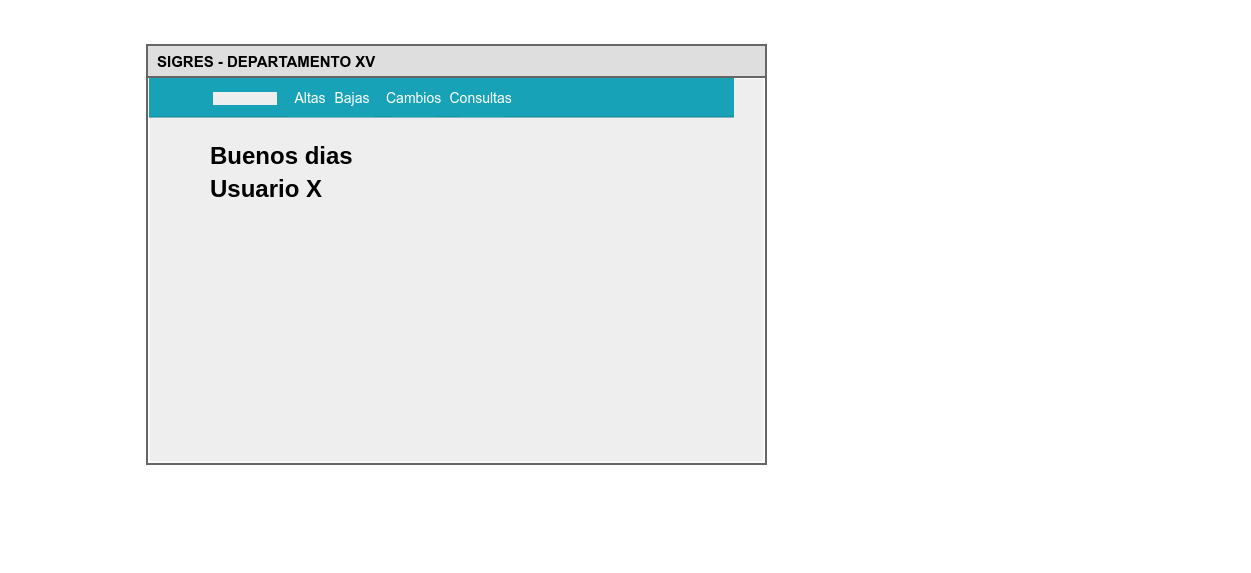
\includegraphics[scale=.3]{iu/mockup1.png}
    \centering
    \caption{B01: Pantalla de bienvenida.}
    \label{fig:b1}
\end{figure}

Una muestra de visualización de datos asociados al espectacular en la figura~\ref{fig:b2}.
\begin{figure}[H]
    \centering
    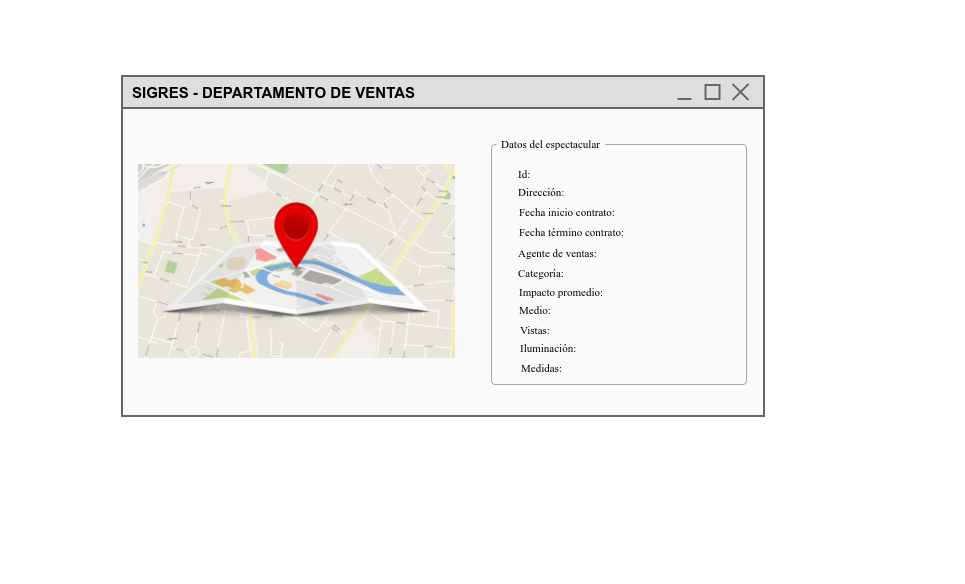
\includegraphics[scale=.4]{iu/mockup2.png}
    \centering
    \caption{B02: Datos del espectacular.}
    \label{fig:b2}
\end{figure}

Un bosquejo de visualización de datos asociados a un empleado en la figura~\ref{fig:b3}.
\begin{figure}[H]
    \centering
    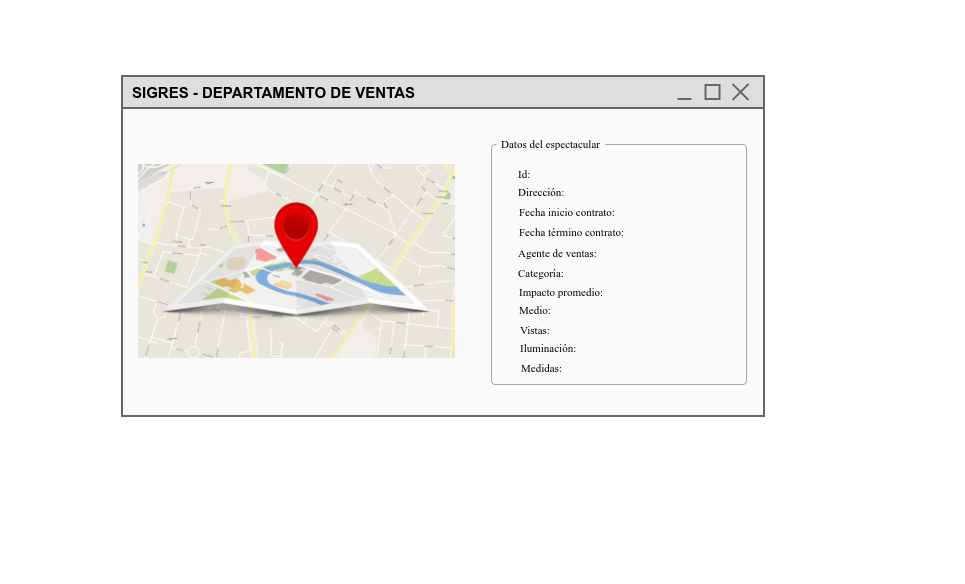
\includegraphics[scale=.4]{iu/mockup2.png}
    \centering
    \caption{B03: Datos del empleado.}
    \label{fig:b3}
\end{figure}

Un bosquejo de alta de empleados en la figura~\ref{fig:b4}. 
\begin{figure}[H]
    \centering
    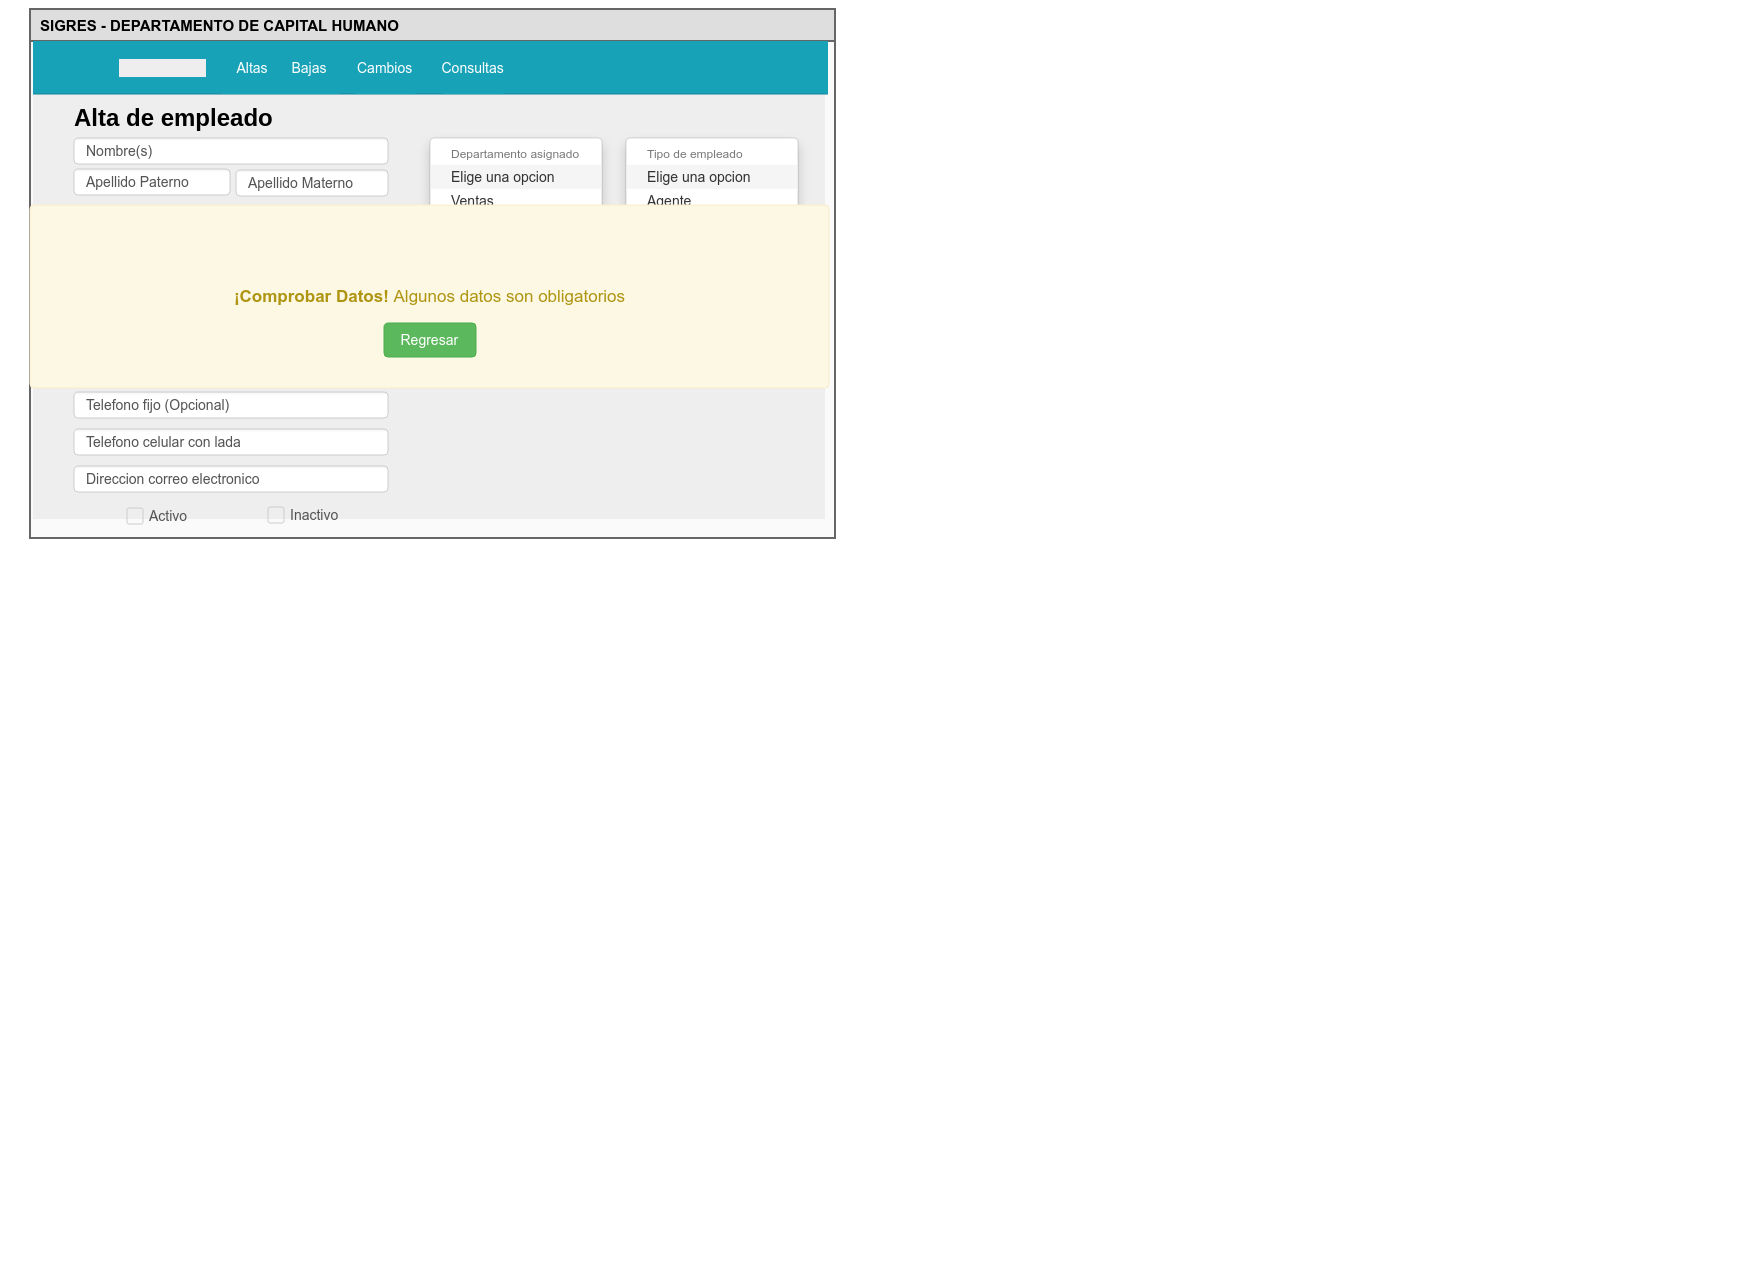
\includegraphics[scale=.4]{iu/mockup4.png}
    \centering
    \caption{B04: Alta de un empleado.}
    \label{fig:b4}
\end{figure}

\section{Alcance}
%---------------------------------------------------------RFX
%---------------------------------------------------------
\subsection{Requerimientos funcionales}
	Los requerimientos funcionales utilizan una clave RFX, donde:
        
\begin{description}
        \item[X] Es un número consecutivo: 1, 2, 3, ...
        \item[RF] Es la clave para todos los {\bf R}equerimientos {\bf F}uncionales.
\end{description}

	Además se usan las abreviaciones que se muestran en la tabla~\ref{tbl:leyendaRF}.
\begin{table}[hbtp!]
        \begin{center}
    \begin{tabular}{|r l|}
            \hline
        {\footnotesize ID} & {\footnotesize\em Identificador del requerimiento.}\\
        {\footnotesize REF} & {\footnotesize\em Referencia del requerimiento.}\\
        {\footnotesize PRI.} & {\footnotesize\em Prioridad}\\
        {\footnotesize MA} & {\footnotesize\em Prioridad Muy Alta.}\\
        {\footnotesize A} & {\footnotesize\em Prioridad Alta.}\\
        {\footnotesize M} & {\footnotesize\em Prioridad Media.}\\
        {\footnotesize B} & {\footnotesize\em Prioridad Baja.}\\
        {\footnotesize MB} & {\footnotesize\em Prioridad Muy Baja.}\\
                \hline
    \end{tabular} 
    \caption{Leyenda para los requerimientos funcionales.}
    \label{tbl:leyendaRF}
        \end{center}
\end{table}
En la tabla ~\ref{tbl:listaRF} se muestran los requerimientos funcionales del sistema a realizar.
<<<<<<< HEAD
\begin{longtable}[H]{m{2cm}m{3cm}m{5cm}m{2cm}m{2cm}}
=======
\begin{longtable}[H]{m{1cm}m{3cm}m{8cm}m{2cm}m{1cm}}
>>>>>>> master
\toprule
\centering \textbf{ID} & \centering  \textbf{Nombre} & \centering \textbf{Descripción} & \centering \textbf{REF}& \centering \textbf{PRI} \tabularnewline
\midrule
\textit{RF1} & \textbf{Alta a un nuevo empleado} & La aplicación deberá permitir el ingreso de un nuevo empleado rellenando los campos correspondientes: nombre completo (compuesto por nombre(s), apellido paterno y apellido materno), dirección (que abarca código postal, calle, número exterior, número interior, colonia, delegación, estado* y referencias), teléfono fijo (opcional), teléfono celular (con lada incluida), dirección de correo electrónico, situación (activo, inactivo), departamento (ventas, jurídico, infraestructura, capital humano) y tipo de empleado (agente, jefe). & RU57, RU61 & MA.\tabularnewline

     \textit{RF2} & \textbf{Identificador de empleado} & A cada empleado registrado se le asignará un identificador único, que será utilizado para identificarle en todos los procesos subsecuentes que se realicen sobre él.& RF1 & MA\tabularnewline
     
     \textit{RF3} & \textbf{Visualización de los datos del empleado} & La aplicación deberá permitir visualizar los datos personales de un empleado específico con base en su identificador. & RU7, RU56, RU57, RU68 & MA\tabularnewline
     
     \textit{RF4} & \textbf{Cambio a un cliente} & La aplicación deberá otorgar la opción para hacer uno o varios cambios a cualesquiera de los campos asociados a un cliente previamente registrado con base a su identificador, sin que se afecte la información que no sea especificada a realizarse un cambio (ni del propio cliente u
otro).& RU13, RU19 & MA\tabularnewline

    \textit{RF5} & \textbf{Alta de un nuevo espectacular} & La aplicación deberá permitir el ingreso de un nuevo espectacular rellenando los campos correspondientes: ubicación en coordenadas (coordenadas reflejadas mediante un mapa), dirección de la ubicación (que abarca código postal, calle, número exterior, colonia, delegación, estado* y referencias), estado, fecha de inicio de contrato de arrendamiento (con formato día/mes/año, opcional), fecha de término de contrato de arrendamiento (con formato día/mes/año, opcional), agente de ventas asignado al contrato de arrendamiento (nombre e identificador, opcional), categoría del espectacular, impacto promedio, medio, vistas, iluminación y medidas.& RU72, RU80 & MA\tabularnewline
    
    \textit{RF6} & \textbf{Identificador del espectacular} & A cada espectacular registrado se le asignará un identificador único, que será utilizado para identificarle en todos los procesos subsecuentes que se realicen sobre él. & RF5 & MA\tabularnewline
    
    \textit{RF7} & \textbf{Visualización de los datos de un espectacular} & La aplicación deberá permitir visualizar la ubicación por coordenadas de cada uno de los espacios publicitarios que posee (mediante un mapa); dirección (que deberá tener los siguientes campos: código postal, calle, número exterior, colonia, delegación, estado* y referencias); fecha de inicio del período de renta (formato: día/mes/año), fecha de término del período de renta (formato: día/mes/año); agente de venta asociada (nombre e identificador); categoría (pudiendo tratarse de: V.I.P., vía primaria y vía secundaria); impacto (números esperados de personas que miran, en promedio y con base a un estudio de mercado previamente realizado y cargado a ella, el espectacular); medio (pantalla o lona); vistas (pudiendo tratarse de: una vista, dos vistas o tres vistas); iluminación (uenta con illuminación, no cuenta con iluminación); medidas (representadas en metros). & RU64, RU73, RU81, RU82 & MA\tabularnewline
    
     \textit{RF8} & \textbf{Cambio a un espectacular} & La aplicación deberá otorgar la opción para hacer uno o varios cambios a cualesquiera de los campos asociados a un espectacular previamente registrado con base a su identificador, sin que se afecte la información que no sea especificada a realizarse un cambio (ni del propio espectacular u otro). & RU65, RU74 & MA\tabularnewline
     
     \textit{RF9} & \textbf{Alta a un nuevo cliente} & La aplicación deberá permitir el ingreso de un nuevo cliente rellenando los campos correspondientes: nombre completo (compuesto por nombre(s), apellido paterno y apellido materno), dirección (que abarca código postal, calle, número exterior, número interior, colonia, delegación, estado* y referencias), teléfono fijo (opcional), teléfono celular (con lada incluida), dirección de correo electrónico, situación (de antaño, nuevo, perdido) y contratos asociados a éste (opcional).& RU11, RU18 & MA\tabularnewline
     
     \textit{RF10} & \textbf{Identificador de cliente} & A cada cliente registrado se le asignará un identificador único, que será utilizado para identificarle en todos los procesos subsecuentes que se realicen sobre él.& RF9 & MA\tabularnewline
     
     \textit{RF11} & \textbf{Visualización de los datos del cliente} & La aplicación deberá permitir visualizar los datos personales de un cliente específico con base en su identificador.& RU12 & MA\tabularnewline
     
     \textit{RF12} & \textbf{Cambio a un cliente} & La aplicación deberá otorgar la opción para hacer uno o varios cambios a cualesquiera de los campos asociados a un cliente previamente registrado con base a su identificador, sin que se afecte la información que no sea especificada a realizarse un cambio (ni del propio cliente u otro).& RU13, RU19 & MA\tabularnewline
     
     \textit{RF13} & \textbf{Alta de una póliza de seguro} & La aplicación deberá permitir el ingreso de una nueva póliza de seguro rellenando los campos correspondientes: nombre de la aseguradora contratada, número de póliza, fecha de inicio de cobertura de la póliza (con formato día/mes/año), fecha de término de cobertura de la póliza (con formato día/mes/año), cobertura de la póliza (monto y siniestros), estado (pudiendo encontrarse vigente, vencida a cambiar, por vencer y vencida registrada) y agente jurídico que tramitó dicha póliza (nombre e identificador).& RU34, RU50 & MA\tabularnewline
     
     \textit{RF14} & \textbf{Identificador de una póliza de seguro} & A cada póliza de seguro registrada se le asignará un identificador único, que será utilizado para identificarle en todos los procesos subsecuentes que se realicen sobre ella. & RF13 & MA \tabularnewline
     
     \textit{RF15} & \textbf{Asociar una póliza de seguro con un espectacular} & Al ingresar pólizas de seguro, toda póliza de seguro estará asociada a un espectacular.& RF13, RF14 & MA \tabularnewline
     
     \textit{RF16} & \textbf{Visualización de una póliza de seguro} & La aplicación deberá permitir visualizar los datos de una póliza de seguro específica con base en su identificador. & RU30, RU46 & MA\tabularnewline
     
     \textit{RF17} & \textbf{Cambio a una póliza de seguro} & La aplicación deberá otorgar la opción para hacer uno o varios cambios a cualesquiera de los campos asociados a una póliza de seguro previamente registrada con base a su identificador, sin que se afecte la información que no sea especificada a realizarse un cambio (ni de la propia póliza u otra). & RU38, RU54 & MA\tabularnewline
     
     \textit{RF18} & \textbf{Alta de un permiso de la Secretaría de Seguridad Pública} & La aplicación deberá permitir el ingreso de un nuevo permiso de la Secretaría de Seguridad Pública rellenando los campos correspondientes: número de permiso, fecha de inicio de cobertura del permiso (con formato día/mes/año), fecha de término de cobertura del permiso (con formato día/mes/año), estado (pudiendo encontrarse vigente, vencido a cambiar, por vencer y vencida registrado) y agente jurídico que tramitó dicho permiso (nombre e identificador).& RU32, RU48, & MA\tabularnewline
     
     \textit{RF19} & \textbf{Identificador de un permiso de la Secretaría de Seguridad Pública} & A permiso de la Secretaría de Seguridad Pública registrado se le asignará un identificador único, que será utilizado para identificarle en todos los procesos subsecuentes que se realicen sobre él. & RF18 & MA\tabularnewline
     
     \textit{RF20} & \textbf{Asociar un permiso de la Secretaría de Seguridad Pública} & Al ingresar permisos de la Secretaría de Seguridad Pública, todo permiso estará asociado a un espectacular. & RF17, RF18 & MA\tabularnewline
     
     \textit{RF21} & \textbf{Visualización de un permiso de la Secretaría de Seguridad Pública} & La aplicación deberá permitir deberá permitir visualizar los datos de un permiso de la Secretaría de Seguridad Pública específica con base en su identificador.& RU28, RU44 & MA\tabularnewline
     
     \textit{RF22} & \textbf{Cambio a un permiso de la Secretaría de Seguridad Pública} & La aplicación deberá otorgar la opción para hacer uno o varios cambios a cualesquiera de los campos asociados a un permiso de la Secretaría de Seguridad Pública previamente registrado con base a su identificador, sin que se afecte la información que no sea especificada a realizarse un cambio (ni del propio permiso u otro). & RU36, RU52  & MA\tabularnewline
     
     \textit{RF23} & \textbf{Alta de un permiso de la Secretaría de Protección Civil} & La aplicación deberá permitir el ingreso de un nuevo permiso de la Secretaría de Protección Civil rellenando los campos correspondientes: número de permiso, fecha de inicio de cobertura del permiso (con formato día/mes/año), fecha de término de cobertura del permiso (con formato día/mes/año), estado (pudiendo encontrarse vigente, vencido a cambiar, por vencer y vencida registrado) y agente jurídico que tramitó dicho permiso (nombre e identificador). & RU33, RU49 & MA\tabularnewline
     
     \textit{RF24} & \textbf{Identificador de un permiso de la Secretaría de Protección Civil} & A permiso de la Secretaría de Protección Civil registrado se le asignará un identificador único, que será utilizado para identificarle en todos los procesos subsecuentes que se realicen sobre él. & RF23 & MA\tabularnewline
     
     \textit{RF25} & \textbf{Asociar un permiso de la Secretaría de Protección Civil} & Al ingresar permisos de la Secretaría de Protección Civil, todo permiso estará asociado a un espectacular. & RF23, RF24 & MA\tabularnewline
     
     \textit{RF26} & \textbf{Visualización de un permiso de la Secretaría de Protección Civil} & La aplicación deberá permitir deberá permitir visualizar los datos de un permiso de la Secretaría de Protección Civil específica con base en su identificador.& RU29, RU45 & MA\tabularnewline
     
     \textit{RF27} & \textbf{Cambio a un permiso de la Secretaría de Protección Civil} & La aplicación deberá otorgar la opción para hacer uno o varios cambios a cualesquiera de los campos asociados a un permiso de la Secretaría de Protección Civil previamente registrado con base a su identificador, sin que se afecte la información que no sea especificada a realizarse un cambio (ni del propio permiso u otro). & RU37, RU53 & MA\tabularnewline
     
     \textit{RF28} & \textbf{Alta de un permiso de la Secretaría de Obras y Servicios} & La aplicación deberá permitir el ingreso de un nuevo permiso de la Secretaría de Obras y Servicios rellenando los campos correspondientes: número de permiso, fecha de inicio de cobertura del permiso (con formato día/mes/año), fecha de término de cobertura del permiso (con formato día/mes/año), estado (pudiendo encontrarse vigente, vencido a cambiar, por vencer y vencida registrado) y agente jurídico que tramitó dicho permiso (nombre e identificador).& RU35, RU51 & MA\tabularnewline
     
     \textit{RF29} & \textbf{Identificador de un permiso de la Secretaría de Obras y Servicios} & A permiso de la Secretaría de Obras y Servicios registrado se le asignará un identificador único, que será utilizado para identificarle en todos los procesos subsecuentes que se realicen sobre él.& RF28 & MA\tabularnewline
     
     \textit{RF30} & \textbf{Asociar un permiso de la Secretaría de Obras y Servicios} & Al ingresar permisos de la Secretaría de Obras y Servicios, todo permiso estará asociado a un espectacular. & RF27, RF28 & MA\tabularnewline
     
     \textit{RF31} & \textbf{Visualización de un permiso de la Secretaría de Obras y Servicios} & La aplicación deberá permitir deberá permitir visualizar los datos de un permiso de la Secretaría de Obras y Servicios específico con base en su identificador.& RU31, RU47 & MA\tabularnewline
     
     \textit{RF32} & \textbf{Cambio a un permiso de la Secretaría de Obras y Servicios} & La aplicación deberá otorgar la opción para hacer uno o varios cambios a cualesquiera de los campos asociados a un permiso de la Secretaría de Obras y Servicios previamente registrado con base a su identificador, sin que se afecte la información que no sea especificada a realizarse un cambio (ni del propio permiso u otro). & RU39, RU55 & MA\tabularnewline
     
     \textit{RF33} & \textbf{Visualización del listado de espectaculares} & La aplicación deberá permitir la visualización de la lista completa de los espectaculares registrados en ella en el momento que se pida. & RU64, RU73 & MA\tabularnewline
     
     \textit{RF34} & \textbf{Visualización del listado de clientes} & La aplicación deberá permitir la visualización de la lista completa de los clientes registrados en ella en el momento que se pida.& RU12, RU16, RU17 & MA\tabularnewline
     
     \textit{RF35} & \textbf{Visualización del listado de empleados} & La aplicación deberá permitir la visualización de la lista completa de los empleados registrados en ella en el momento que se pida.& RU56, RU60 & MA\tabularnewline
     
     \textit{RF36} & \textbf{Visualización del listado de permisos y pólizas asociados a un espectacular} & La aplicación deberá permitir la visualización de la lista completa de los peermisos y pólizas registrados en ella asociados a un espectacular mediante su identificador en el momento que se pida.& RU28-RU31, RU44-RU47 & MA\tabularnewline
     
     \textit{RF37} & \textbf{Póliza vencida registrada}& Únicamente el Titular de Jurídico podrá actualizar el estado de una póliza de seguros asociada a un espectacular a "vencida registrada".& RU42 & MA\tabularnewline
     
     \textit{RF38} & \textbf{Permiso vencido registrado}& Únicamente el Titular de Jurídico podrá actualizar el(los) estado(s) de un(varios) permiso(s) (cualesquiera de los tres emitidos por: Secretaría de Seguridad Pública de la Ciudad de México, Secretaría de Obras y Servicios de la Ciudad de México, Secretaría de Protección Civil de la Ciudad de México) asociado a un espectacular a "vencido registrado".& RU40, RU41, RU43 & MA\tabularnewline
     
     \textit{RF39} & \textbf{Espectacular descontinuado} & Únicamente el Jefe de Infraestructura podrá actualizar el estado de un espectacular a "descontinuado".& RU66 &MA\tabularnewline
     
     \textit{RF40} & \textbf{Empleado inactivo} & Únicamente el Jefe de Capital Humano podrá actualizar el estado de un empleado de cualesquiera de los departamentos a "inactivo".& RU59 & MA\tabularnewline
     
     \textit{RF41} & \textbf{Cliente perdido} & Únicamente el Gerente de Ventas podrá actualizar el estado de un cliente a "perdido". & RU14 & MA\tabularnewline
     
\caption{Requerimientos funcionales del sistema}
\label{tbl:listaRF}
\bottomrule
<<<<<<< HEAD
\end{longtable}
=======
\end{longtable}
>>>>>>> master

%---------------------------------------------------------
%---------------------------------------------------------RNFX
\subsection{Requerimientos no funcionales}
\subsubsection{Plataforma}
\begin{itemize}
    \item {Sistema gestor de bases de datos: MySQL Server  versión 5.0}
    \item {Lenguaje de programación de propósito general: PHP versión 7.0}
    \item {Navegador web: Cualesquiera de las versiones de Google Chrome, Mozilla Firefox y/o Safari}
    \item {Memoria de Acceso Aleatorio: 4GB mínimo, 8GB recomendado}
    \item {Procesador: Cuatro núcleos a 2.4GHz (recomendado)}
\end{itemize}

En el diagrama de despliegue~\ref{fig:plataforma} podemos visualizar exactamente las mismas especificaciones.
\begin{figure}[H]
    \centering
    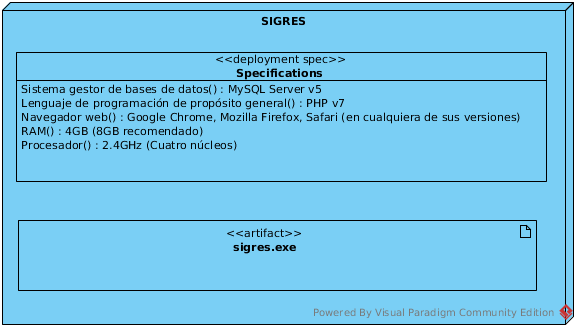
\includegraphics[scale=.7]{images/plataforma.png}
    \centering
    \caption{DRNF01: Plataforma del sistema.}
    \label{fig:plataforma}
\end{figure}

\subsubsection{Interacción del Usuario}
\begin{itemize}
    \item {}
\end{itemize}

\subsubsection{Procesos del negocio}
En la siguiente tabla~\ref{tbl:listaUP} se muestran los usuarios contemplados para el diseño del sistema y los procesos que se modelaron.
\begin{longtable}[H]{m{4cm}m{8cm}}
    \toprule
    \centering \textbf{Usuario} & \centering  \textbf{Procesos} \tabularnewline
    \midrule
    \textbf{Gerente de Ventas} & Alta de un nuevo cliente, cambios a un cliente existente, búsqueda de un cliente, visualización datos de todo el listado de clientes, eliminación de datos de un cliente perdido.\tabularnewline
    \textbf{Agente de ventas} & Alta de un nuevo cliente, cambios a un cliente existente, búsqueda de un cliente, visualización datos de todo el listado de clientes.\tabularnewline
    \textbf{Titular de Jurídico} & Alta de un nuevo permiso (cualesquiera de los tres emitidos por: Secretaría de Seguridad Pública de la Ciudad de México, Secretaría de Obras y Servicios de la Ciudad de México, Secretaría de Protección Civil de la Ciudad de México), cambios a un permiso registrado (cualesquiera de los tres emitidos por: Secretaría de Seguridad Pública de la Ciudad de México, Secretaría de Obras y Servicios de la Ciudad de México, Secretaría de Protección Civil de la Ciudad de México), búsqueda de un permiso registradi (cualesquiera de los tres emitidos por: Secretaría de Seguridad Pública de la Ciudad de México, Secretaría de Obras y Servicios de la Ciudad de México, Secretaría de Protección Civil de la Ciudad de México), visualización datos de todo el listado de permisos vigentes asociado a un espectacular, alta de una nueva póliza de seguros de un espectacular, cambios  a una póliza de seguros de un espectacular,  visualización datos de póliza de seguros vigente asociada a un espectacular, eliminación de datos de una póliza de seguros, eliminación de datos de un permiso cualesquiera de los tres emitidos por: Secretaría de Seguridad Pública de la Ciudad de México, Secretaría de Obras y Servicios de la Ciudad de México, Secretaría de Protección Civil de la Ciudad de México).\tabularnewline
    \textbf{Agente jurídico} & Alta de un nuevo permiso (cualesquiera de los tres emitidos por: Secretaría de Seguridad Pública de la Ciudad de México, Secretaría de Obras y Servicios de la Ciudad de México, Secretaría de Protección Civil de la Ciudad de México), cambios a un permiso registrado (cualesquiera de los tres emitidos por: Secretaría de Seguridad Pública de la Ciudad de México, Secretaría de Obras y Servicios de la Ciudad de México, Secretaría de Protección Civil de la Ciudad de México), búsqueda de un permiso registradi (cualesquiera de los tres emitidos por: Secretaría de Seguridad Pública de la Ciudad de México, Secretaría de Obras y Servicios de la Ciudad de México, Secretaría de Protección Civil de la Ciudad de México), visualización datos de todo el listado de permisos vigentes asociado a un espectacular, alta de una nueva póliza de seguros de un espectacular, cambios  a una póliza de seguros de un espectacular,  visualización datos de póliza de seguros vigente asociada a un espectacular.\tabularnewline
    \textbf{Jefe de Infraestructura} & Alta de un nuevo espectacular, cambios a un espectacular existente, búsqueda de un espectacular, visualización datos de todo el listado de espectaculares, eliminación de un espectacular.\tabularnewline
    \textbf{Agente de Infraestructura} & Alta de un nuevo espectacular, cambios a un espectacular existente, búsqueda de un espectacular, visualización datos de todo el listado de espectaculares.\tabularnewline
    \textbf{Jefe de Capital Humano} & Alta de un nuevo empleado, cambios a un empleado existente, visualización datos de todo el listado de empleados, eliminación de un empleado.\tabularnewline
    \textbf{Agente de Capital Humano} & Alta de un nuevo empleado, cambios a un empleado existente, visualización datos de todo el listado de empleados. \tabularnewline

\caption{Usuarios y procesos contemplados}
\label{tbl:listaUP}
\bottomrule
<<<<<<< HEAD
\end{longtable}
=======
\end{longtable}
>>>>>>> master


\subsubsection{Información y datos}

\subsubsection{Propiedades del software}
\begin{itemize}
    \item Verificabilidad
    \item Correctitud
    \item Confiabilidad
    \item Amigabilidad
    \item Mantenibilidad
    \item Reparabilidad
    \item Evolucionabilidad
\end{itemize}

%---------------------------------------------------------
